\documentclass[cs4size,a4paper,adobefonts,openany]{ctexbook}
\usepackage[colorlinks=true,linkcolor=black]{hyperref}
\usepackage{indentfirst}
\usepackage[a4paper,left=2.5cm,right=2.5cm,bottom=2.5cm,top=2.5cm]{geometry}
\usepackage{amsmath,amsthm,amssymb}
\usepackage{fontspec}
\setmainfont{Palatino}
\pagestyle{plain}
\punctstyle{kaiming}
\usepackage{unicode-math}
\setmathfont{Asana Math}

\newtheorem{defn}{定义}
\newtheorem{thm}{定理}
\newcommand{\pname}[1]{\underline{#1}}
\numberwithin{equation}{section}
\CTEXsetup[number=\thechapter]{chapter}
\begin{document}
\title{\bfseries Regular Polytopes 的学习笔记}
\author{王盛颐}
\date{}
\maketitle
\setcounter{page}{1}
\chapter{POLYGONS AND POLYHEDRA}
\section{Regular polygons}
假设有 $p$ 个点 $A_1,A_2,\dots,A_p$,那么 $p$ 边形($p$-gon)被定义为连
接这些点的 $p$ 条直线段 $A_1A_2,A_2A_3,\dots,A_pA_1$ 形成的环路。这些线
段和点分别被称为多边形的\pname{边}和\pname{顶点}。目前我们假定所有的边
都不彼此穿插。如果一个多边形所有的顶点都共面,则我们称其为\pname{平面}
多边形,否则称为\pname{斜}多边形。

一个平面多边形将它所在的平面划分为两个区域,面积有限的称为\pname{内部}。
我们通常将这个内部也视作多边形的组成部分,和顶点、边一样。这时平面多边
形可以有另外一个定义,定义为由 $p$ 个不同直线段围成的单连通区域(这里单
  连通区域的意思是区域内任意简单闭曲线都可以连续收缩成一个点)。

有一类平面多边形,特点是任意一条边所在的直线都不穿过多边形内部,这类多
边形特别重要,我们称之为\pname{凸} $p$ 边形,可以用(笛卡尔坐标下)
$p$ 个线性不等式来描述:
\[
a_kx+b_ky \leq c_k\qquad (k=1,2,\dots,p)
\]
这组不等式必须是一致的,没有冗余的,且能据此得到一个有限的积分:
\[
\iint\text{d}x\text{d}y
\]
(这就是多边形的面积)。

一个平面多边形若每条边都相等则被称为等边的,若每个角都相等则被称为等角
的。当 $p>3$ 时,一个平面 $p$ 边形可能等边但不等角,如菱形;也可能等角但
不等边,如长方形。若一个平面 $p$ 边形既等角又等边,则被称之为\pname{正
  则的} (regular),也叫\pname{正} $p$ 边形,记为 $\{p\}$。如 $\{3\}$
是指正三角形,$\{4\}$ 表示正方形,$\{5\}$ 表示正五边形。

很容易看出一个正多边形有一个\pname{中心点},从中心点出发到各个角距离相
等为 ${_0R}$,到各条边距离相等为 ${_1R}$。这意味着两个同心圆,分别是正多边
形的外接圆和内切圆。

有时可以将 $p$ 边形的边认作是首尾相接的 $p$ 个向量。将这些向量的起点并
在一处,则相邻向量的夹角就等于 $p$ 边形的外角,于是 $p$ 边形的外角和为
$2\pi$。那么 $\{p\}$ 的每个外角大小都是 $2\pi/p$,所以每个内角的大小是
\begin{equation}
  \label{eq:innerAngle}
  (1-\frac{2}{p})\pi
\end{equation}

这也可以从图 \ref{fig:pentagon} 中的直角三角形 $O_2O_1O_0$ 看出来。
$O_2$ 是中心,$O_1$ 是一条边的重点,$O_0$ 是这条边的一个端点。直角在
$O_1$ 处,$O_2$ 处的角度显然是 $\pi/p$。若边长为 $2l$ 则我们有:
\[
O_0O_1=l,\quad O_0O_2={_0R}, \quad O_1O_2={_1R}
\]
因此有
\begin{equation}
  {_0R}=l\csc\frac{\pi}{p}\qquad {_1R}=l\cot\frac{\pi}{p}
\end{equation}

那么 $\{p\}$ 的面积就是这样 $p$ 个三角形的面积和:
\begin{equation}
  C_p = pl\cdot {_1R} = pl^2\cot\frac{\pi}{p}
\end{equation}
周长则是
\begin{equation}
  S=2pl
\end{equation}

\begin{figure}[htbp]
  \centering 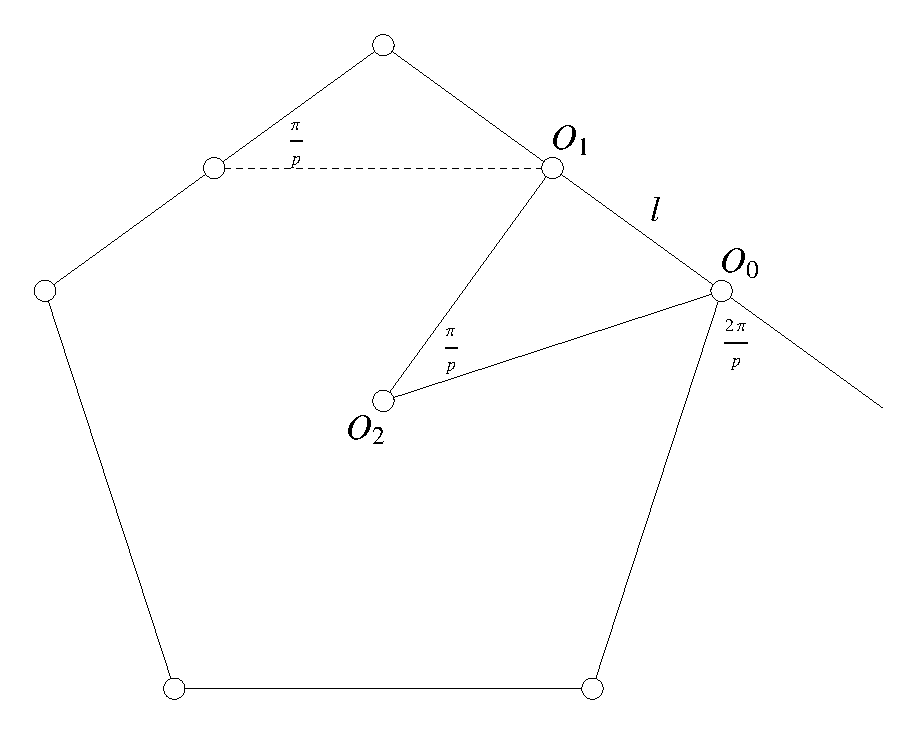
\includegraphics[width=0.7\textwidth]{images/pentagon}
  \caption{正 $p$ 边形的角度长度关系} \label{fig:pentagon}
\end{figure}

当 $p$ 无限增长下去,则 $S/{_0R}$ 和 $S/{_1R}$ 都会渐渐接近 $2\pi$ (阿基米
  德当年就是这么算圆周率的,他计算用的 $p=96$)。

我们也可以计算出 $\{p\}$ 各个顶点的笛卡尔坐标为
\[
\left({_0R}\cos\frac{2k\pi}{p},{_1R}\sin\frac{2k\pi}{p}\right)\qquad(k=0,1,\dots,p-1)
\]

把这些坐标看作复平面上的点,那么外接圆半径 ${_0R}=1$ 的 $\{p\}$ 的顶点可
以认为是分圆方程
\begin{equation}
  z^p=1
\end{equation}
的根 $e^{2k\pi i/p}$。

有时需要扩展 $p$ 边形的定义,允许多边形的边为曲线。比如有时候可能会考虑
\pname{圆多边形},它的边都是球面上大圆的圆弧,这种情况下可以有二边形。

\section{Polyhedra}
一个\pname{多面体}可以被定义为由有限个互相连接的平面多边形构成的集合。
具体连接方式是这样的:每个多边形的每一条边都和且仅和另外一个多边形共享,
围绕每一个顶点的多边形都只能形成一条回路(这是为了排除掉两个棱锥共享一
  个顶点的情形)。构成多面体的这些平面多边形称之为多面体的\pname{面},
这些多边形的边称之为该多面体的\pname{棱}。目前为止我们都假定所有的面都
不彼此穿插。

如上定义的一个多面体形成了一个封闭曲面,将所在空间划分为两个区域,体积
有限的称为\pname{内部}。我们通常将内部也视为多面体的组成部分。不妨假定
一个多面体有 $N_2$ 个面,$N_1$ 条棱和 $N_0$ 个顶点。

有一类多面体,特点是任意一个面所在的平面都不穿过多面体内部。这类多面体
特别重要,我们称之为\pname{凸}多面体,可以用(笛卡尔坐标下)的一组不等
式来描述:
\[
a_kx+b_ky+c_kz \leq d_k\qquad (k=1,2,\dots,N_2)
\]
这组不等式必须是一致的,没有冗余的,且能据此得到一个有限积分:
\[
\iiint\text{d}x\text{d}y\text{d}z
\]
(这就是多面体的体积)。

有些多面体和包围它们的多边形一样常见。一个 $p$ 边形和与其不共面的一个点
可以用 $p$ 个三角形连接起来,形成一个\pname{棱锥}(pyramid)。两个全等的
$p$ 边形可以被 $p$ 个长方形连起来形成一个直\pname{棱柱}(prism)。将直棱
柱两个 $p$ 边形的其中一个做同一平面内的旋转,使其顶点(边)正对应另一个
$p$ 边形的边(顶点),将这两个多边形用 $2p$ 个三角形连起来就形成了一个
\pname{反棱柱}(anti-prism)。

一个\pname{四面体}(tetrahedron) 是以三角形为基底的棱锥,它的面由四个三
角形构成,任意一个都能做基底。当这四个都是等边三角形时,我们就得到了一
个\pname{正}四面体,这是五种柏拉图立体中最简单的一个。另外四个分别是立
方体(cube)、正八面体(octahedron)、正十二面体(dodecahedron) 和正二十面体
(icosahedron)。

\section{The five Platonic Solids}

一个凸多面体被称为是\pname{正} (regular) 多面体,当且仅当它的面都是正多
边形,且每个顶点都被同样数量的多边形围绕。若这个正多面体的面是 $\{p\}$,
且每个顶点被 $q$ 个多边形围绕,则将这个正多面体记为 $\{p,q\}$

正多面体 $p$ 和 $q$ 的取值可以用下面的方法推算出来:正多面体一个顶点处
有 $q$ 个围绕着的平面角,根据 \eqref{eq:innerAngle} 可知,每个角大小为
$(1-2/p)\pi$。因为这是一个凸多边形,可以想像从这个顶点处沿任意一条棱剪
开后这个角可以平铺在平面上,所以这 $q$ 个角大小之和不超过 $2\pi$,于是
有$1-2/p<2/q$,也即
\begin{equation}
  \frac{1}{p}+\frac{1}{q}>\frac{1}{2}
\end{equation}
或为 $(p-2)(q-2)<4$,因此 $\{p,q\}$ 无非只有下面 $5$ 种取值:
\[
\{3,3\},\quad\{3,4\},\quad\{4,3\},\quad\{3,5\},\quad\{5,3\}
\]
正四面体 $\{3,3\}$ 我们已经构造出来了。这 $5$ 种取值只是正多面体的必要
条件,未必是充分条件,还得真正构造出来才能说是充要条件。

将两个底面全等的棱锥底贴底的粘在一起,就得到了一个由 $2p$ 个三角形围成
的\pname{双棱锥} (dipyramid)。若这个共同的基底是 $\{p\}$ ($p<6$),那么
通过调整棱锥的高度,可以让这些三角形都变成全等的等边三角形。当 $p=4$ 时,
每个顶点都被 4 个全等的等边三角形围绕。此时任意对顶的顶点都能被视为双棱
锥的两极。这样的多面体就是正八面体 $\{3,4\}$。

通过调整直棱柱的高度,可以让它所有的侧面都变成正方形,若基底也是正方形,
我们就得到了立方体 $\{4,3\}$,它的每个面都可以看做直棱柱的基底。

类似的,通过调整一个基底是 $\{p\}$ 的反棱柱的高度,可以让其侧边的 $2p$
个三角形都变成全等的等边三角形。若 $p=3$,我们就再次得到了正八面体。若
$p=4$ 或 $5$,则在它的两个基底上再各加一个棱锥后,通过调整棱锥的高度,
可以得到由 $4p$ 个全等的等边三角形围成的凸多面体。当 $p=5$ 时,每个顶点
周围都围绕着 $5$ 个三角形,这就是正二十面体 $\{3,5\}$。

第 5 个柏拉图立体就没有上述这么简单的构造方法了。可以取 6 个全等的正五
边形,令其中一个五边形被另外五个五边形完全包围起来,形成一个碗状的结构。
“碗”的边沿是一个锯齿状的十边形。两个这样的“碗”对合在一起,边沿彼此相合,
如此就得到了正十二面体 $\{5,3\}$。

\section{Graphs and maps}
一个多面体的顶点和棱构成了一个特殊的图,由 $N_0$ 个结点,$N_1$ 条边或者
叫\pname{分支}(未必要是直的)。如一个结点属于 $q$ 个分支,那么显然有
\begin{equation}
  \sum q = 2N_1
\end{equation}
上述求和取遍 $N_0$ 个结点。对一个连通图来说,则必须有
\begin{equation}
  \label{eq:connectIneq}
  N_1\geq N_0-1
\end{equation}

一个图被称为\pname{包含}另外一个图,当且仅当这个图可由另一个图添加边或
者添加边和顶点得到。一个图可能包含由 $p$ 个分支与 $p$ 个结点构成的圈,
如 $p$ 边形 ($p\geq 2$)。

一个不包含圈的图称为\pname{森林},若这个不包含圈的图连通,则称其为
\pname{树}。对树来说,\eqref{eq:connectIneq} 中的等号成立:
\begin{equation}
  N_1=N_0-1
\end{equation}
这是因为一个树可以从任意结点开始构造,每次新添加一个分支,分支另一端是
个新的结点。
\end{document}
